%\documentclass[10pt]{beamer}
\documentclass[10pt,handout]{beamer}
\usepackage[english]{babel}
% % \usepackage[backend=biber, style=authoryear-icomp]{biblatex}
\resetcounteronoverlays{exx}
\usepackage{mdframed}
\usepackage{tikz}
\usepackage{blindtext}
\usepackage{tipa}
% \usepackage{cgloss4e}
% \usepackage{gb4e}
% \usepackage{qtree}
\usepackage{cancel}
\usepackage{wrapfig}
\usepackage{soul}
\usepackage{enumerate}
\usepackage{longtable}
\graphicspath{ {.} } % declaramos donde estan las imagenes
\usepackage[labelformat=simple]{subcaption} % para varias imagenes juntas
\renewcommand\thesubfigure{(\alph{subfigure})}
\usepackage[utf8]{inputenc}
\usepackage{amsmath}
\usepackage{amsfonts} % simbolos como el I de matriz identidad
\usepackage{bm}
\usepackage{graphicx} % paquete para ver imagenes
\usepackage{setspace}
\usepackage[T1]{fontenc}
\usepackage{parskip}
\usepackage{color}
\usepackage{framed}
\usetheme{Copenhagen}
\definecolor{frenchblue}{rgb}{0.0, 0.45, 0.73} % ESTE!!!!
\definecolor{myblue1}{RGB}{35,119,189}
\definecolor{myblue2}{RGB}{95,179,238}
\definecolor{myblue3}{RGB}{129,168,207}
\definecolor{myblue4}{RGB}{26,89,142}

\setbeamercolor{block body}{bg=frenchblue!50}
\setbeamercolor*{structure}{fg=frenchblue,bg=blue}
\setbeamertemplate{frametitle}[default][center]
\setlength{\parskip}{12pt}
\useoutertheme{infolines} % me comia mucho espacio de la otra fgorma
\makeatother
\setbeamertemplate{footline}
{
  \leavevmode%
  \hbox{%
  \begin{beamercolorbox}[wd=.3\paperwidth,ht=2.25ex,dp=1ex,center]{author in head/foot}%
    \usebeamerfont{author in head/foot}\insertshortauthor
  \end{beamercolorbox}%
  \begin{beamercolorbox}[wd=.6\paperwidth,ht=2.25ex,dp=1ex,center]{title in head/foot}%
    \usebeamerfont{title in head/foot}\insertshorttitle
  \end{beamercolorbox}%
  \begin{beamercolorbox}[wd=.1\paperwidth,ht=2.25ex,dp=1ex,center]{date in head/foot}%
    \insertframenumber{} / \inserttotalframenumber\hspace*{1ex}
  \end{beamercolorbox}}%
  \vskip0pt%
}
\newcommand{\floor}[1]{\lfloor #1 \rfloor}

\makeatletter
\setbeamertemplate{navigation symbols}{}
%\setbeameroption{show notes}
\setbeameroption{hide notes}


\usepackage{hyperref}

\title[CHOCO]{Client-optimized Algorithms and Acceleration for Encrypted Compute Offloading}
\author[Matias Mazzanti]{Matias Mazzanti}




\institute{}
\date{04 of April de 2023}


\begin{document}

\begin{frame}

\maketitle

\end{frame}


\section{Organization}
%%%%%%%%%%%%%%%%%%%%%%%%%%%%%%%%%%%%%%%%%%%%%%%%%%%%%%%%%%%%%%%%%%%%%%%%%%%%%%%%%%%%%%%%%%%%%%%%%%%%
% 15 - 20 slides (good ones..)


%Brief summary
%what is the problem the paper is trying to solve
%what are the key ideas of the paper
%what is the key contribution to literature at the time
%what are the most important things you take out from it
%
%- Strenghts
%does the paper solve the problem well?
%
%- Weaknesses
%Critically! Search weakness not bad things.
%
%
%
%
%    Introduction (1 slide)
%    Research Questions/Hypotheses (1 slide)
%    Literature Review/Theory (1 slide)
%    Methods & Data Collection (1 slide)
%    Data Presentation/Findings (3-5 slides)
%    Conclusion (1 slide)

\begin{frame}
    \frametitle{CHOCO-TACO}

    CHOCO is New approach for FHE.

    Accelerate Encryption and Decryption (the client side).

    Use the client to refresh the noise.

    Use the client to do nonlinear operations.

    New algorithm for minimice computation cost.

    CHOCO-TACO is a hardware accelerator for this.
\end{frame}
%%%%%%%%%%%%%%%%%%%%%%%%%%%%%%%%%%%%%%%%%%%%%%%%%%%%%%%%%%%%%%%%%%%%%%%%%%%%%%%%%%%%%%%%%%%%%%%%%%%%
\begin{frame}[noframenumbering]
    \frametitle{Schedule}
\begin{columns}
    \column{0.5\textwidth}
    Part 1:
    \begin{itemize}
        \item What is HE?
        \item What is FHE?
        \item Schemes
        \item Math notation
    \end{itemize}

    \column{0.5\textwidth}
    Part 2:
    \begin{itemize}
        \item What is HE?
        \item What is FHE?
        \item Schemes
        \item Math notation
    \end{itemize}
\end{columns}

\end{frame}




%% hacer una especie de entre cortito de que es?

%%%%%%%%%%%%%%%%%%%%%%%%%%%%%%%%%%%%%%%%%%%%%%%%%%%%%%%%%%%%%%%%%%%%%%%%%%%%%%%%%%%%%%%%%%%%%%%%%%%%
\section{Introduction}
\begin{frame}
\frametitle{What is HE?}


    Homomorphic Encrpytion (HE) $\rightarrow$ form of encryption. Early 80s
\vspace{-0.3cm}

    Operate \textbf{directly} with encrypted data (without the need of decrypt).
\vspace{0.3cm}
  \begin{columns}
    \column{0.5\textwidth}
Typical use case:
\begin{itemize}
    \item Client encrypted his data with his own secret key.
    \item Send this and the public key to the server.
    \item Server operates with out decryption (e.g. Machine Learning).
    \item Server send back the result in the encryption form.
    \item Client decrypts the result with the secret key.
\end{itemize}


\column{0.5\textwidth}

\begin{figure}[h!]
    \centering
    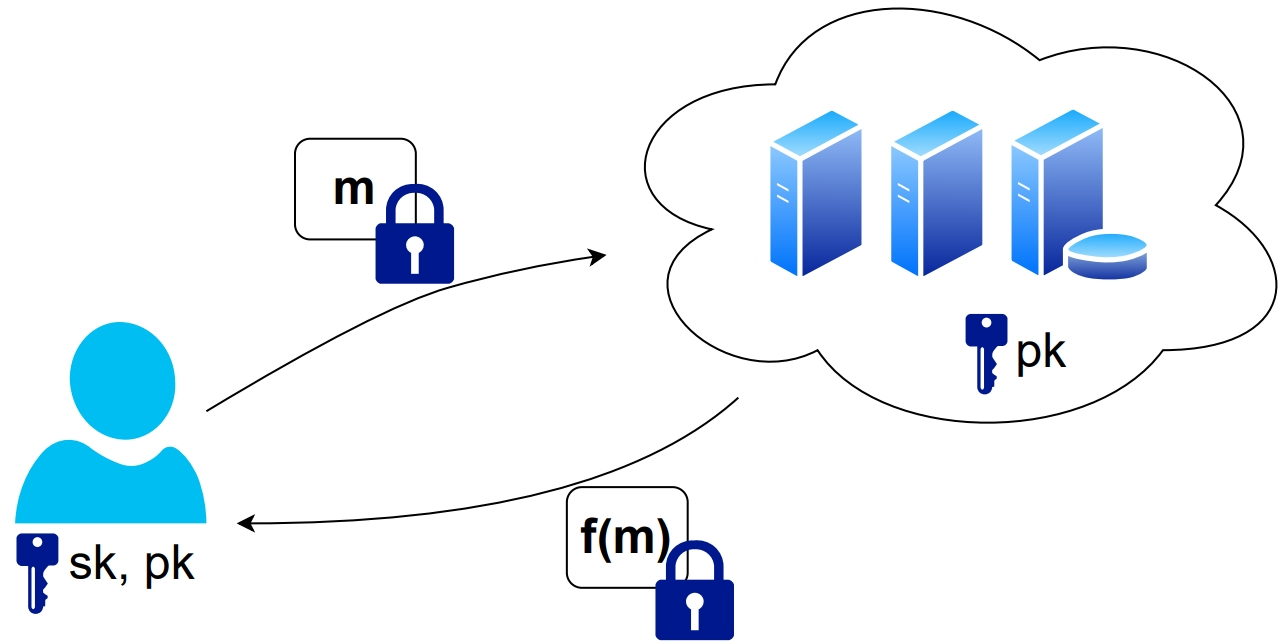
\includegraphics[scale=0.1]{fhe.jpg}
    \caption{Paper:https://ia.cr/2022/657}
\end{figure}
\end{columns}
 \vspace{-0.3cm}


Potentially very useful for cloud computing use.
 \vspace{-0.3cm}

 \pause
    \textbf{Present}: Orders of magnitude \textbf{slower} for real use.


\end{frame}

% ACA PONER COMO ES CLIENT-AIDED?

%%%%%%%%%%%%%%%%%%%%%%%%%%%%%%%%%%%%%%%%%%%%%%%%%%%%%%%%%%%%%%%%%%%%%%%%%%%%%%%%%%%%%%%%%%%%%%%%%%%%


\begin{frame}
    \frametitle{FHE}
  \begin{columns}
    \column{0.5\textwidth}
      In general, HE schemes use \texttt{Ring Learning With Errors} (RLWE) that  adds some sort of noise (error) to the encryption.

\vspace{0.3cm}
    This noise grows in each operation (particularly with multiplications).

\vspace{0.3cm}
      If the noise is too big will be undecryptable.
    \column{0.5\textwidth}
        \begin{figure}[h!]
            \centering
            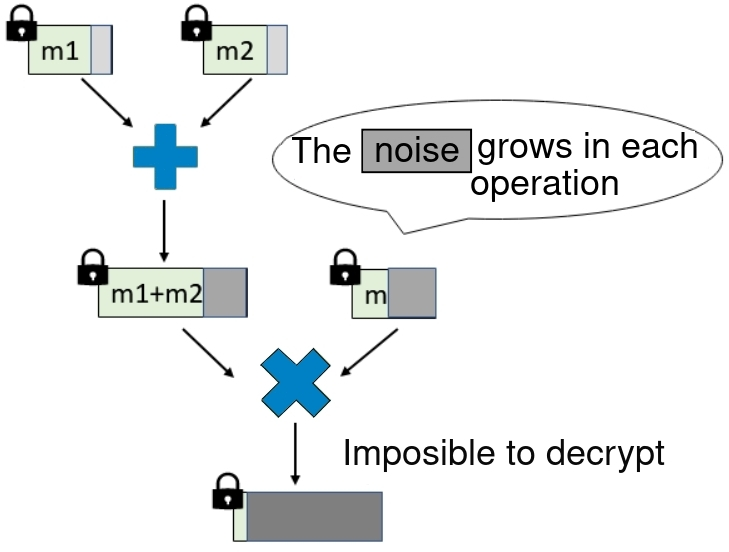
\includegraphics[scale=0.2]{multNoise.jpg}
        \end{figure}



\end{columns}

    Fully Homomorphic Encryption (FHE): Unlimited number of operations. In this type of schemes
    it use \texttt{Bootstrapping} that are techniques that refresh this error.

    Even slower!!!

    \textbf{Other problem}: Only linear operations!
\end{frame}

%%%%%%%%%%%%%%%%%%%%%%%%%%%%%%%%%%%%%%%%%%%%%%%%%%%%%%%%%%%%%%%%%%%%%%%%%%%%%%%%%%%%%%%%%%%%%%%%%%%%


\begin{frame}
    \frametitle{Schemes}

    Many schemes. \textbf{Warning}: Many acronyms!!!

    Popular schemes by types:
    \begin{itemize}
        \item Operations on integers: BFV and BGV.
        \item Operations on real numbers: CKKS.
        \item Operations on Boolean gates: FHEW and THFHE.
    \end{itemize}

    \textbf{Paper}: BFV.

    \textbf{Implementations}: Residue Number System (RNS) (stay with 64bits arithmetic's), and SIMD arithmetic (batching).

\end{frame}

%%%%%%%%%%%%%%%%%%%%%%%%%%%%%%%%%%%%%%%%%%%%%%%%%%%%%%%%%%%%%%%%%%%%%%%%%%%%%%%%%%%%%%%%%%%%%%%%%%%%


\begin{frame}
    \frametitle{BFV}

Works in a Polynomial Ring domain.

\textbf{Ring}: a set with addition, subtraction and multiplication. (and other property's, commutative, associative, etc).

This operations of elements in a ring return elements in the ring $\rightarrow$ take modulus.

\textbf{Parameters}: are application-specific and desire security.

\begin{itemize}
    \item $\lambda$ security level. $\sim$ $2^\lambda$ operation to decrypt with prob 1.
    \item N will be the degree of the Polynomials (N-1).
    \item q and t will be the mod of the coefficients.
\end{itemize}


\end{frame}


%%%%%%%%%%%%%%%%%%%%%%%%%%%%%%%%%%%%%%%%%%%%%%%%%%%%%%%%%%%%%%%%%%%%%%%%%%%%%%%%%%%%%%%%%%%%%%%%%%%%

% quizas menos.
\begin{frame}
\frametitle{BFV Primitives}

    Basic Primitives (simplified):
\begin{itemize}
    \item ParamGen($\lambda$)$\rightarrow$ Params.
    \item KeyGen(Params) $\rightarrow$ SK, PK, EvalK (each is a tuple of two polynomials)
   \item Encrypt(PK, m) $\rightarrow$ c (tuple of two polynomials)
    \item Decrypt(SK, c) $\rightarrow$ m
    \item EvalAdd(c$_1$, c$_2$) $\rightarrow$ c$_3$ (tuple of two polynomials)
    \item EvalMult(c$_1$, c$_2$) $\rightarrow$ c$_{mul}$ (tuple of three polynomials)
    \item Relinerize(c$_{mul}$, EvalK) $\rightarrow$ c$_{mul}$' (tuple of two polynomials)
\end{itemize}

\end{frame}
%%%%%%%%%%%%%%%%%%%%%%%%%%%%%%%%%%%%%%%%%%%%%%%%%%%%%%%%%%%%%%%%%%%%%%%%%%%%%%%%%%%%%%%%%%%%%%%%%%%%


\begin{frame}
    \frametitle{Bootstrapping tradeoff}

    Approach 1:

    Know how many operations are needed (depth level)

    Bigger scheme parameters $\approx$ bigger noise budget $\approx$ slower computation.

    Approach 2:

    Use Bootstrapping us needed.


    Approach 3 (Paper):

    Use the client to unencrypte an encrpyt again (refresh the noise).
\end{frame}



%%%%%%%%%%%%%%%%%%%%%%%%%%%%%%%%%%%%%%%%%%%%%%%%%%%%%%%%%%%%%%%%%%%%%%%%%%%%%%%%%%%%%%%%%%%%%%%%%%%%

% combinarla con la de los parametros.
\begin{frame}
\frametitle{Parameters}

The parameters depends in the security level needed and amount of operations that will made.


Some usual parameters to get the sense of what we are doing:

N = 8192, 16384, 32768.

    q = $2^{218}$,   $2^{438}$,  $2^{881}$. (bigger q, bigger noise budget)

t  << q.

% que significa q/t


\end{frame}
%%%%%%%%%%%%%%%%%%%%%%%%%%%%%%%%%%%%%%%%%%%%%%%%%%%%%%%%%%%%%%%%%%%%%%%%%%%%%%%%%%%%%%%%%%%%%%%%%%%%

% combinarla con la de los parametros.
\begin{frame}
\frametitle{Operations}

    \textbf{Keys generations}: Sample 3 polynomials. Then two polynomail multiplication, Two additions and two modulus.

    \textbf{Encryption}: Sample 3 polynomials. Then two polynomial multiplication, one scalar multiplication, three additions and two modulus.

    \textbf{Decryption}: similar to Encryption.

    \textbf{Multiplication + Relinerize}: Six polynomial multiplications, three additions and five modulus.

   Multiplications make the noise grow a lot.

    \textbf{RNS}: naive explanation, slipt a ciphertext of more than 64bits in $k$ chunks and operates in that way.

\end{frame}


%%%%%%%%%%%%%%%%%%%%%%%%%%%%%%%%%%%%%%%%%%%%%%%%%%%%%%%%%%%%%%%%%%%%%%%%%%%%%%%%%%%%%%%%%%%%%%%%%%%%

\begin{frame}
\frametitle{Recap}

    \textbf{Rembember!} All things are high degree polynomials with huge coefficient.

Each homomorphic operation is $10^3 \sim 10^6$ times slower than unencrypted.
\pause

Large footprint in memory.
An encrypted date can occupy $10^5$ more space.

\pause
    The schemes are iterative, operating many time with each data specialy Bootstrapping (CHOCO don't use it).

        \begin{figure}[h!]
            \centering
            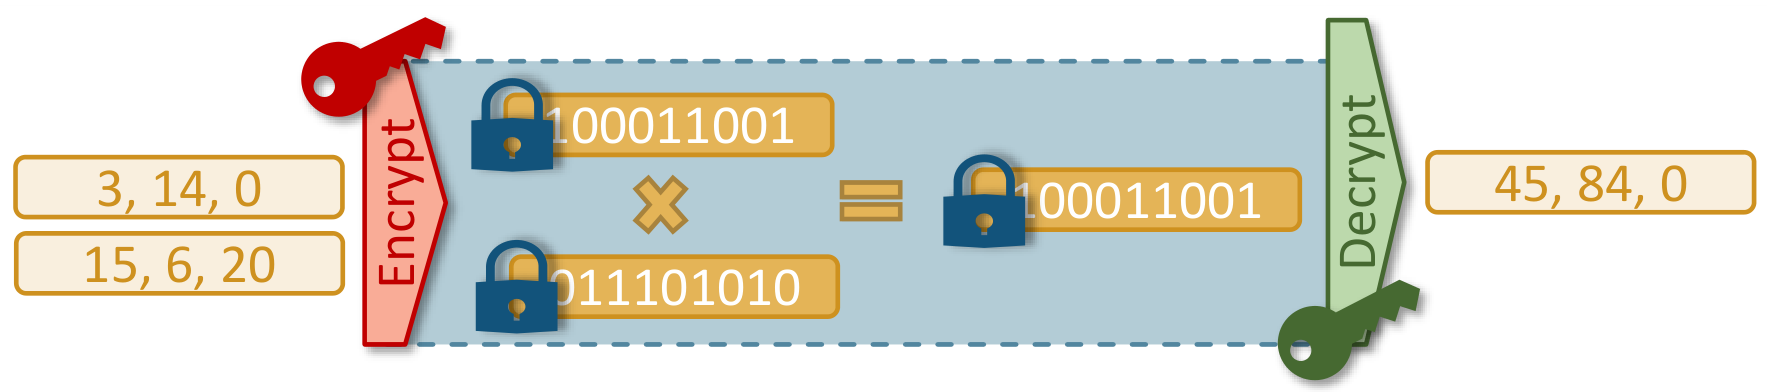
\includegraphics[scale=0.8]{workflow.png}
        \end{figure}
    \centering
        SIMD example

\end{frame}
%%%%%%%%%%%%%%%%%%%%%%%%%%%%%%%%%%%%%%%%%%%%%%%%%%%%%%%%%%%%%%%%%%%%%%%%%%%%%%%%%%%%%%%%%%%%%%%%%%%%


\begin{frame}
\frametitle{Research}

    Usual way of increase performance:  accelerating the server part.
\begin{itemize}\itemsep-0.7em
   \item Accelerating the polynomial multiplication:
    For these they use Number Theoretic Transform (NTT), a Discrete Fourier Transform (DFT) over a ring.
   \item New schemes.
   \item New upgrades in the schemes (like RNS).
   \item New methods of Bootstrapping.
   \item Algorithms implementations, like packed ones (concatenate multiple plaintexts).
   \item Hardware Acceleration (GPUs, FPGA, specific designs).
\end{itemize}

    \textbf{Linearity problem}: Aproximate with polynomial expantions.
\end{frame}
%%%%%%%%%%%%%%%%%%%%%%%%%%%%%%%%%%%%%%%%%%%%%%%%%%%%%%%%%%%%%%%%%%%%%%%%%%%%%%%%%%%%%%%%%%%%%%%%%%%%


\begin{frame}
\frametitle{New approach}
Accelerate the client side, specialy encryption and decryption.

CHOCO: \textbf{C}lient-aided \textbf{H}E for \textbf{O}paque \textbf{C}ompute \textbf{O}ffloading.

Is a client-aided HE: operate by using the client multiple times.

Prior systems of these type also focus on accelerating the server part.

% para que y cuando se utiliza el rotacional redundancy
    Minimice the client costs.
\begin{itemize}\itemsep-0.7em
    \item Reduces ciphertext size $\rightarrow$ reducing the cost of comunication.
    \item New algorithm: rotational redundancy $\rightarrow$ reduces computation costs.
    \item Reduction of parameters values $\rightarrow$ reduces computation and comunication costs.
    \item Hardware acceleration for client: CHOCO-TACO.
\end{itemize}


\end{frame}



%%%%%%%%%%%%%%%%%%%%%%%%%%%%%%%%%%%%%%%%%%%%%%%%%%%%%%%%%%%%%%%%%%%%%%%%%%%%%%%%%%%%%%%%%%%%%%%%%%%%

\section{Research}

\begin{frame}
\frametitle{Motivation}


\begin{figure}
    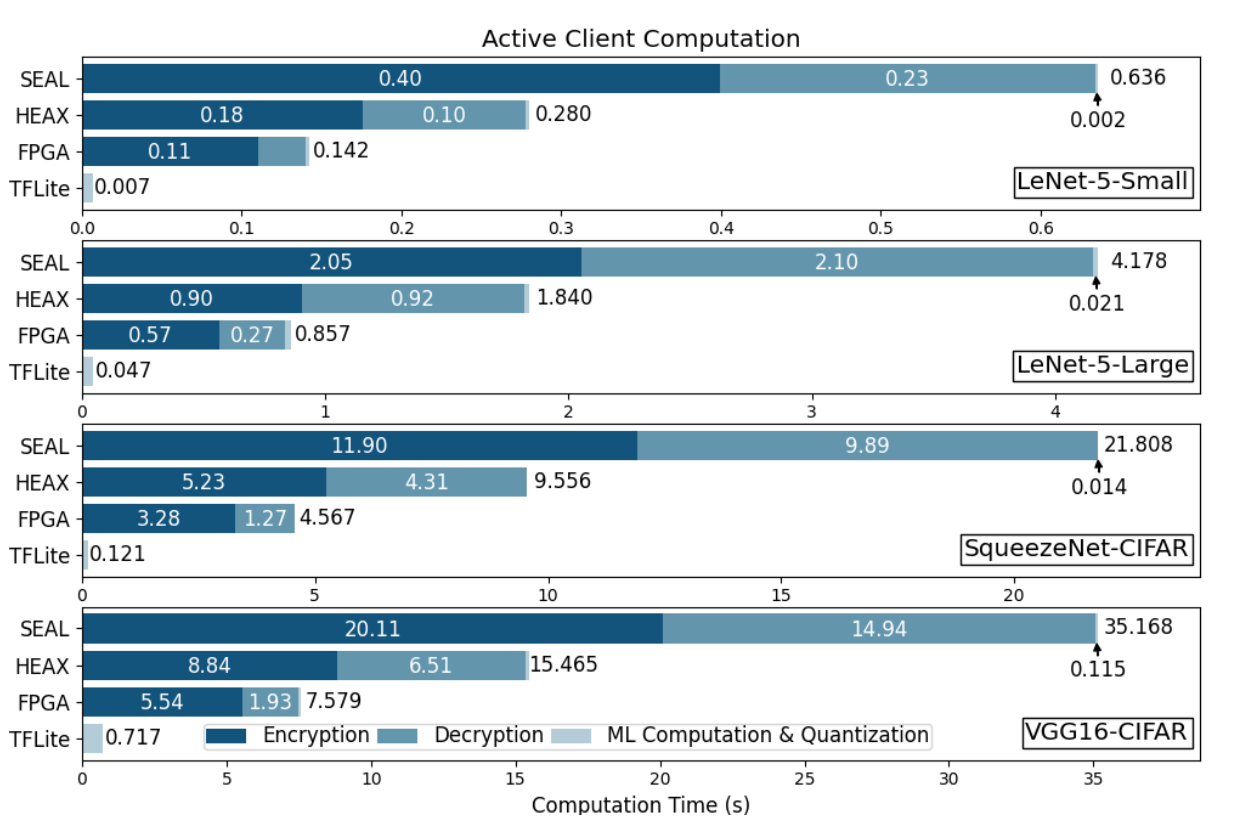
\includegraphics[width=0.45\textwidth]{motivation.png}
\end{figure}


The most clear example: DNN inference.

Before: No client itermiediate comunication $\rightarrow$ adapt networks architectre and approximations of non-linear operations.

    Problems: Fast noise acumulation, large HE parameters, big ciphertext (more costly to process and communication)

CHOCO:
\begin{itemize}
    \item Client-aided $\rightarrow$ offload linear convolution and fully-conected layers to HE server.
    \item Send intermediate reuslts to the client to perform non-linear operations and refresh noise.
    \item Supports unmodified networks with arbitrary activation functions.
\end{itemize}

Larger client cost!

    CHOCO minimize this cost (with also CHACO-TACO).

\end{frame}


%%%%%%%%%%%%%%%%%%%%%%%%%%%%%%%%%%%%%%%%%%%%%%%%%%%%%%%%%%%%%%%%%%%%%%%%%%%%%%%%%%%%%%%%%%%%%%%%%%%%


\begin{frame}
\frametitle{}
<<<<<<< HEAD

Quizas solo contar que vieron que el 99\% del tiempo se lo lleva el encrypt y decrypt

y que ademas NTT y esas cosas llevan solo el 60\% del tiempo.

QUEDA LA DUDA DE quanitzar 4bits.... SI pasan de 8 bits a 4 bits, super agresivo.
pero parece que para estas cosas funciona y reduce mucjho el tamaño del cifrado

Evaluation of client costs - communication and computation.

Four DNN models with a client using TFLite
\begin{figure}
    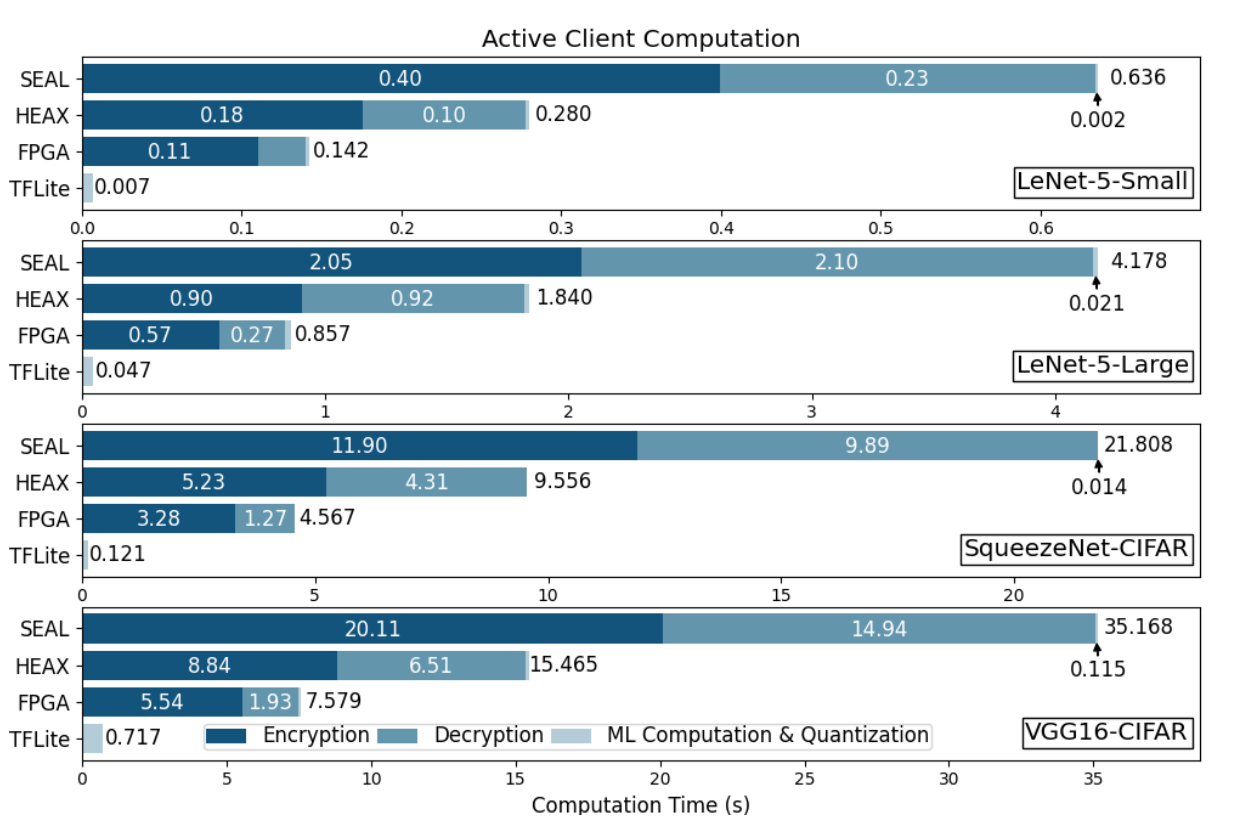
\includegraphics[width=0.45\textwidth]{motivation.png}
\end{figure}



\end{frame}


%%%%%%%%%%%%%%%%%%%%%%%%%%%%%%%%%%%%%%%%%%%%%%%%%%%%%%%%%%%%%%%%%%%%%%%%%%%%%%%%%%%%%%%%%%%%%%%%%%%%


\begin{frame}
\frametitle{Rotational Redundancy}

Packed HE algorithms $\rightarrow$  rearrange ecrypted vectors $\rightarrow$ rotations and multiplications.

Noise grows a lot!

%Convolutions use a lot of rotations. Explica como lo usaron...


New algorithm! Rotational Redundancy.

    Client appends redundant values to the plaintext (before the encryption).
\begin{figure}
    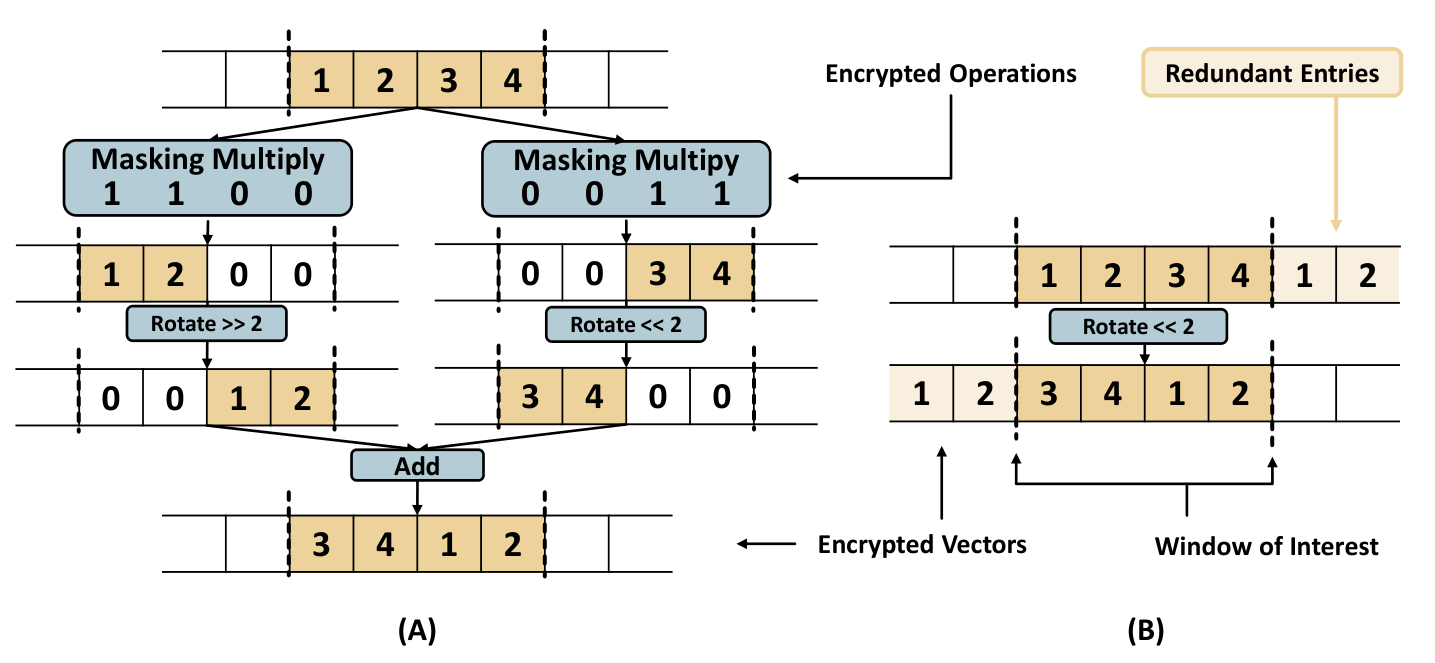
\includegraphics[width=0.65\textwidth]{rotation.png}
\end{figure}

Exploits the fact that the client  always decrypt, unpack, repack and encrypt.

So client discard redundant data adds new values for the next operation.

Tipically the redundancy is a small fraction of the total vector size.
\end{frame}

%%%%%%%%%%%%%%%%%%%%%%%%%%%%%%%%%%%%%%%%%%%%%%%%%%%%%%%%%%%%%%%%%%%%%%%%%%%%%%%%%%%%%%%%%%%%%%%%%%%%


\begin{frame}
\frametitle{Rotational Redundancy}
uso y beneficios del rotational

\end{frame}
%%%%%%%%%%%%%%%%%%%%%%%%%%%%%%%%%%%%%%%%%%%%%%%%%%%%%%%%%%%%%%%%%%%%%%%%%%%%%%%%%%%%%%%%%%%%%%%%%%%%


\begin{frame}
\frametitle{}
Taco

\begin{figure}
    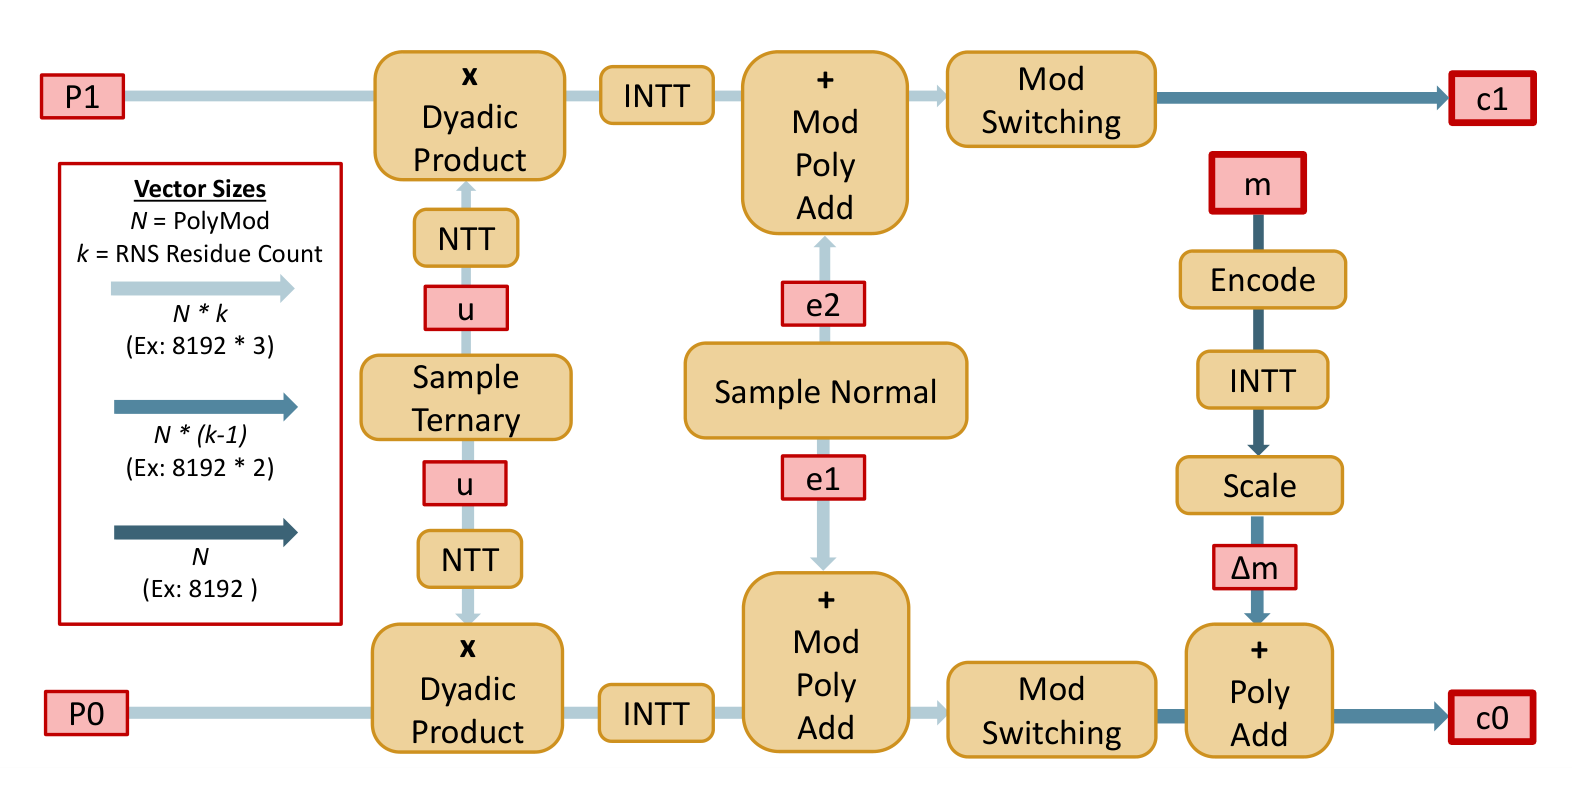
\includegraphics[width=0.55\textwidth]{pipeline.png}
\end{figure}

\end{frame}
%%%%%%%%%%%%%%%%%%%%%%%%%%%%%%%%%%%%%%%%%%%%%%%%%%%%%%%%%%%%%%%%%%%%%%%%%%%%%%%%%%%%%%%%%%%%%%%%%%%%


\begin{frame}
\frametitle{}
Taco

\begin{figure}
    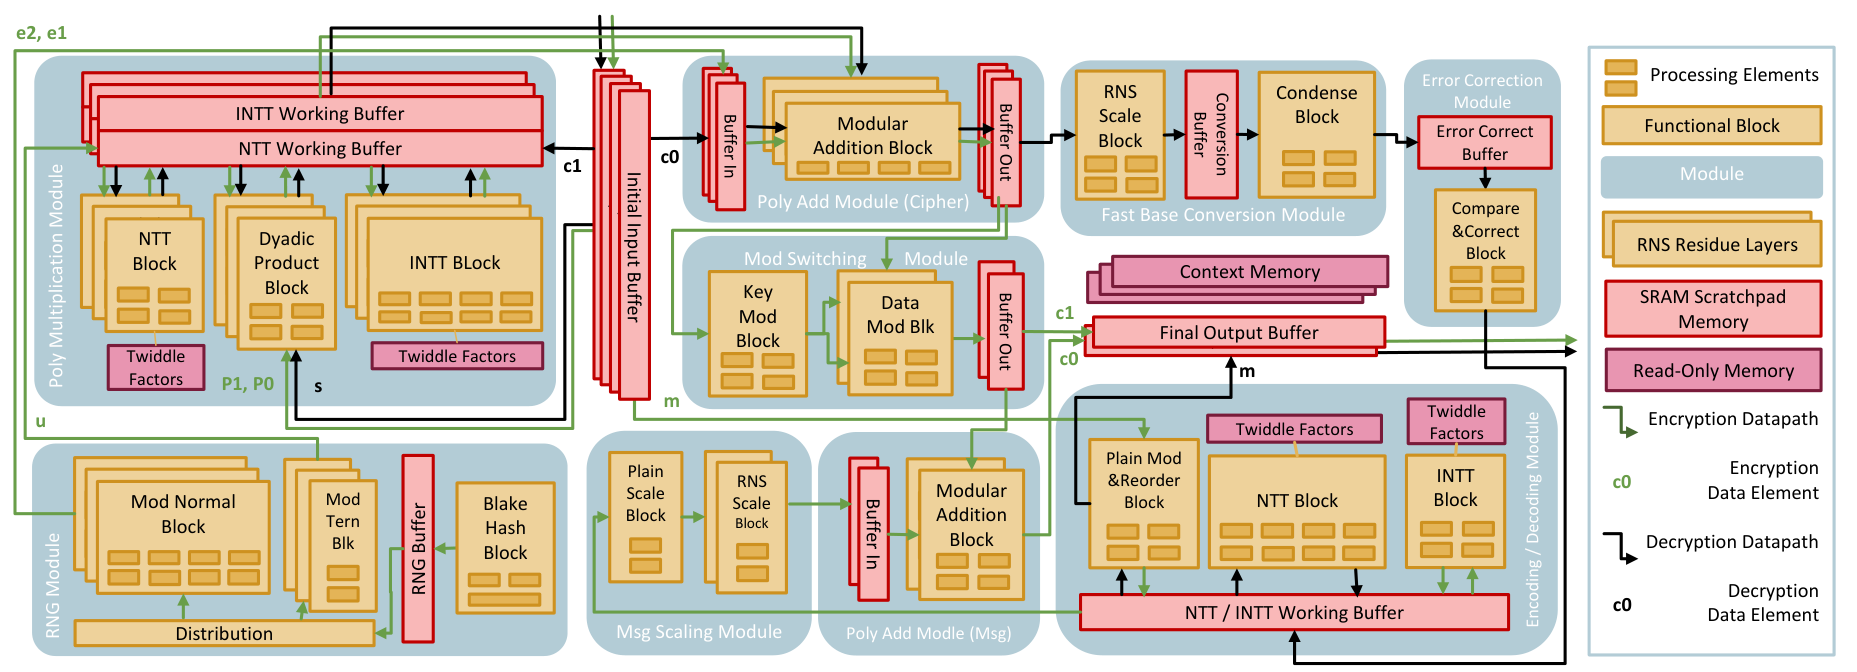
\includegraphics[width=0.85\textwidth]{architecture.png}
\end{figure}

\end{frame}


%%%%%%%%%%%%%%%%%%%%%%%%%%%%%%%%%%%%%%%%%%%%%%%%%%%%%%%%%%%%%%%%%%%%%%%%%%%%%%%%%%%%%%%%%%%%%%%%%%%%


\begin{frame}
\frametitle{}
design space
\end{frame}

%%%%%%%%%%%%%%%%%%%%%%%%%%%%%%%%%%%%%%%%%%%%%%%%%%%%%%%%%%%%%%%%%%%%%%%%%%%%%%%%%%%%%%%%%%%%%%%%%%%%


\begin{frame}
\frametitle{}
evaluation
\end{frame}

%%%%%%%%%%%%%%%%%%%%%%%%%%%%%%%%%%%%%%%%%%%%%%%%%%%%%%%%%%%%%%%%%%%%%%%%%%%%%%%%%%%%%%%%%%%%%%%%%%%%


\begin{frame}
\frametitle{}
communiation reduces
\end{frame}

%%%%%%%%%%%%%%%%%%%%%%%%%%%%%%%%%%%%%%%%%%%%%%%%%%%%%%%%%%%%%%%%%%%%%%%%%%%%%%%%%%%%%%%%%%%%%%%%%%%%


\begin{frame}
\frametitle{}
Taco client compute
\end{frame}

%%%%%%%%%%%%%%%%%%%%%%%%%%%%%%%%%%%%%%%%%%%%%%%%%%%%%%%%%%%%%%%%%%%%%%%%%%%%%%%%%%%%%%%%%%%%%%%%%%%%


\begin{frame}
\frametitle{}
chaco comunication
\end{frame}
%%%%%%%%%%%%%%%%%%%%%%%%%%%%%%%%%%%%%%%%%%%%%%%%%%%%%%%%%%%%%%%%%%%%%%%%%%%%%%%%%%%%%%%%%%%%%%%%%%%%

\section{Conclution}
\begin{frame}
\frametitle{}
conlcution
\end{frame}
%%%%%%%%%%%%%%%%%%%%%%%%%%%%%%%%%%%%%%%%%%%%%%%%%%%%%%%%%%%%%%%%%%%%%%%%%%%%%%%%%%%%%%%%%%%%%%%%%%%%


\begin{frame}
\frametitle{}
conclution
\end{frame}
%%%%%%%%%%%%%%%%%%%%%%%%%%%%%%%%%%%%%%%%%%%%%%%%%%%%%%%%%%%%%%%%%%%%%%%%%%%%%%%%%%%%%%%%%%%%%%%%%%%%


\begin{frame}
\frametitle{}
\Huge

\begin{center}
   Questions?
\end{center}
\end{frame}


%%%%%%%%%%%%%%%%%%%%%%%%%%%%%%%%%%%%%%%%%%%%%%%%%%%%%%%%%%%%%%%%%%%%%%%%%%%%%%%%%%%%%%%%%%%%%%%%%%%%

%%%%%%%%%%%%%%%%%%%%%%%%%%%%%%%%%%%%%%%%%%%%%%%%%%%%%%%%%%%%%%%%%%%%%%%%%%%%%%%%%%%%%%%%%%%%%%%%%%%%

% Quizas al pedo.
\begin{frame}[noframenumbering]
\frametitle{Math notation}
BFV, BGV and CKKS works with ciphertex  $\in \mathcal{R}_q =\mathbb{Z}_q[X]/(X^N+0)$

$\mathbb{Z}[X]$ = Set of Polynomials with integer coefficients.

$\mathbb{Z}_q[X]$ = Set of Polynomials with integer coefficients mod q.

$\mathbb{Z}_q[X]/(X^N+0)$ = The Polynomials degree N-1.


\end{frame}
%%%%%%%%%%%%%%%%%%%%%%%%%%%%%%%%%%%%%%%%%%%%%%%%%%%%%%%%%%%%%%%%%%%%%%%%%%%%%%%%%%%%%%%%%%%%%%%%%%%%

%quizas tampoco
\begin{frame}[noframenumbering]
\frametitle{Workflow}

    Encryption has two phases:
\begin{itemize}
    \item From an integer m to plaintext
    \item From plain text to ciphertext c.
\end{itemize}


\begin{figure}
    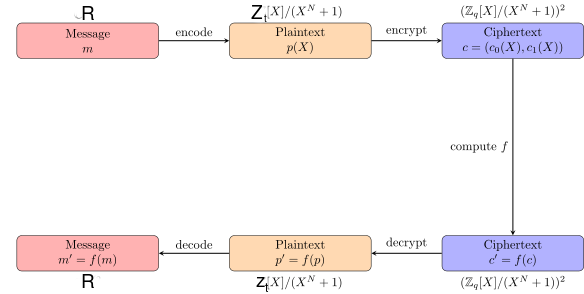
\includegraphics[width=0.85\textwidth]{bfv-diagram.png}
\end{figure}


\end{frame}


\begin{frame}[noframenumbering]

    \frametitle{Encryption}

    Encryption has two phases:

    - From an integer m to plaintext M $\rightarrow$ Easy, one way: binary representation as Polynomial coefficient.

    - From plaintext to ciphertext using $PK = (PK_1, PK_2)$:

    \begin{itemize}
        \item Sample a polynomial $u$ from $\mathcal{R}_2$.
        \item Sample polynomial errors $e_1$ and $e_2$ form a Gaussian distribution.
        \item Calculate scaling factor $\triangle = \lfloor q/t\rfloor $
        \item Encryption of plaintext M is $C=(C_1, C_2)$
    \end{itemize}
    %
    \begin{align}
        &C_1 = [PK_1 * u + e_1 + \triangle M ]_q\nonumber \\
        &C_2 = [PK_2 * u + e_2]_q\nonumber
    \end{align}


\end{frame}
%%%%%%%%%%%%%%%%%%%%%%%%%%%%%%%%%%%%%%%%%%%%%%%%%%%%%%%%%%%%%%%%%%%%%%%%%%%%%%%%%%%%%%%%%%%%%%%%%%%%


\begin{frame}[noframenumbering]

    \frametitle{Multiplication}

    High computational cost:
    \vspace{-0.15cm}

    $C_{mul} = C*C' = (C_1*C_1',C_1*C_2'+C_2*C_1', C_2*C_2') = (C_a,C_b,C_c)$
    \vspace{-0.15cm}

    \textbf{Problem}: If we keep multiplying, the number of Polynomials will grow and will be needed
    the squared of the SK.

    \textbf{Relinerize}:
    $EvalK = (-PK_1+SK^2, PK_2)$

    $C_{mul} = (C_a, C_b, C_c)\approx ([C_a+EvalK_1*C_c]_q, [C_b+EvalK_2*C_c]_q)$

    \textbf{Other problem}: high noise growth: we are multiplying the errors of the two ciphertexts, the result error
    grows a lot!
    \vspace{-0.1cm}

    \textbf{Solution}: \vspace{-0.3cm}
    \begin{itemize} \vspace{-0.2cm}
        \item Select the lowest parameters for the ''exact'' amount  of operations needed (HE). \vspace{-0.2cm}
            \vspace{-0.25cm}
        \item Use Bootstrapping  (FHE). Even more demanding (multiple multiplications like $C_{mul}$).
    \end{itemize}
\end{frame}

\end{document}

